\chapter{Proposed Study}
\label{chap:study}

In the original scope of this research a study was proposed which would effectively aim to prove whether or not the TieSim application is an effective teaching tool. As the research progressed, however, it became clear that the development of TieSim would take far too long to allow for an in depth study to take place. For this reason, the current chapter has been included to outline a proposed study to accompany this research in the future. All of the included materials were submitted to, and approved by Appalachian State's IRB for Spring 2015. As such, the proposed study can be carried out exactly as outlined, and one should expect a quick approval again from IRB in the future.

\section{Procedures}
\label{sec:procedures}

The overall structure of this study is quite simple. Participants will be gathered individually by the PI in a controlled environment. For the purposes of the initial IRB submission the location was defined as a private study room in the Belk Library, though any secure office setting would work fine. Inside the study location will be a table with a mannequin and a couple of men's neckties, as well as a computer and the Oculus Rift DK2 headset with mounted Leap Motion V2 unit. The computer will serve two purposes, the first of which is to run the actual TieSim application, and the second is to securely record the participant's data (see section 5.5: Privacy). Each participant would be expected to commit an average forty minutes of their time to the study. 

Upon the participant's arrival at the study location, they will be walked through the consent forms (see section 5.3: Consent), and will then be introduced to the study itself. Following this they will be shown how to wear the Oculus Rift DK2, and will then be immersed in the TieSim application. The simulation will take no more than 30 minutes, and will teach the participants how to tie a men's necktie in virtual reality. Participants will only have to sit and look around while using their hands as primary input to control the simulation. After the simulation is complete participants will remove the headset and will then be re-oriented into real life.

Following the simulation, participants will be given a real necktie and be asked to tie it on the aforementioned mannequin. Their success or failure will be recorded (see section 5.6: Data), along with how long it took them to achieve success or give up. Additional follow up questions will be asked to further identify the participant's experience with the application, and finally the study will be concluded. After all of the study's procedures have been completed, participants will have their name entered into a prize raffle to win a \$50 Amazon Gift Card.

\section{Recruitment}
\label{sec:recruit}

The ideal number of participants sought for this study should be in the range of 150 participants. Of course, it can often be difficult to find such a large number of volunteer participants in a short time, and thus in the original documents submitted for IRB approval, only 30 participants were specified. The targeted participant population is defined as college students (only eighteen or older). The targeted population is an appropriate group to bear the burdens of this research, and they are also a subset of the population most likely to receive the benefits of this research. The targeted participant population must also not already possess the skill the study aims to teach, and additionally if one gets motion sick easily they will be discouraged from participating (see section 5.4: Risks and Benefits). 

Students will be recruited through an email containing the materials found in Appendix A.1. This email will be sent to as many departments as possible, and will also be printed out as a flyer and attached to departmental bulletin boards throughout campus. Participants will be encouraged to volunteer as they will be entered into a fair raffle drawing for a \$50 Amazon Gift Card for completing the simulation and answering the follow-up questions (see section 5.1: Procedures).

\section{Consent}
\label{sec:consent}

As discussed earlier participants will be given a consent form upon their arrival to the study. A copy of this form can be found in Appendix A.2. Each participant will be walked through the entire form by the present researcher before participating in the study. At any point before, during, or after this step of the study, if participants want to ask questions or are unsure of the study's procedures, they will be encouraged to ask about the process. After being walked through the consent form, participants will need to sign the form in order to begin participating in the study, though there are no known factors that might interfere with informed consent.

\section{Risks and Benefits}
\label{sec:risks}

As part of the official IRB approval from Appalachian State, this study was determined to involve minimal risk to participants. However, even though this study received such a classification it should be noted that there do exist some potential risks for this study (albeit minimal ones). The primary source of potential risk lies with the known side effect of motion sickness that can occur while immersed in VR. This side effect almost always occurs when the person being immersed in VR has a tendency to get motion sick easily from other sources (i.e. roller coasters, ski lifts, or motor vehicles). If a participant gets motion sick easily, it is entirely possible that they could feel lightheaded and dizzy as a result of the TieSim application. In such a case the participant should immediately take off the headset and be excused from the study to protect their health. Due to the health risks involved with VR, it is standard procedure to include a health warning at the beginning of all applications, and TieSim is no exception as seen in Figure~\ref{figure:f_health}.

\begin{figure}
  \centering
  %\begin{picture}
  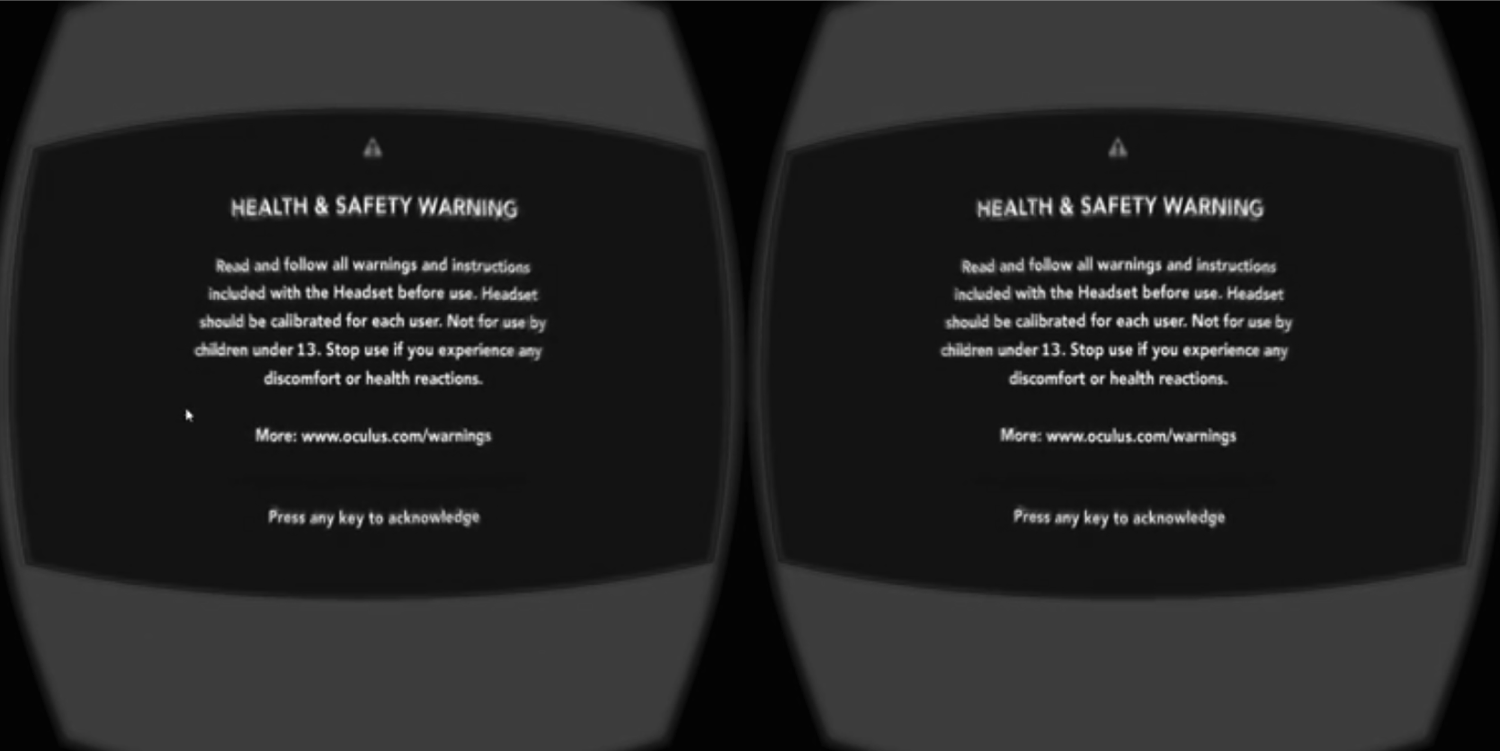
\includegraphics[scale=.55]{img_health}
  %\end{picture}
  \caption{Screenshot of TieSim's health warning at launch.}
  \label{figure:f_health}
\end{figure}
%Figure~\ref{figure:f_dk1}

It is of critical importance, that if a participant were to feel motion sick during the simulation, that the above measures be taken immediately. Furthermore, their data should not be kept as it is incomplete and does not help better the study. Only the researcher present will have knowledge of any identifying characteristics after the data is removed from the computer.

The potential benefits of the study should be quite clear: as a result of the study participants will possibly have gained the ability to tie a men's necktie. As well, society may benefit from the study in that this research uniquely applies cutting edge virtual technology to an educational simulation. Depending on what the results of the study dictate, this research could go a long way to rationalize this new technology as a valid educational tool.

\section{Privacy}
\label{sec:Privacy}

The privacy of each participant is of utmost importance throughout the study, and it can't be stressed enough how important it is to keep the individual participant's data and identity secure. Only the principle researcher can be present at the time of the study, and all data must be recorded on a single computer behind the principle researcher's login and password. Additionally, the data recorded during the study (see section 5.6: Data), must be stored in an encrypted excel .CSV file. The only data kept will be non-identifying demographic information (i.e. age, sex, major), and the results of the study along with the follow-up questions. The data kept in the excel file will be entered into randomized rows, to ensure that the row value does not correlate to the participant's number (which will not be kept). 

\section{Data}
\label{sec:data}

After completing the simulation portion of the study, participants will be expected to attempt to replicate the skill taught in VR, and will then be asked a series of follow up questions. These questions can be found in Appendix A.3 and focus on a range of metrics. The most simple items recorded will be metrics such as how long it took them to tie the tie, how long they spent in VR, and simple demographics information. As well, participants will be asked to answer a handful of opinion questions regarding their experience in the VR simulation, and how effective they perceived the technology to be. These questions will be answered on a scale from 1-5, where 1 correlates with strongly disagree, 2 with disagree, 3 with undecided, 4 with agree, and 5 with strongly agree.